\documentclass[tikz]{standalone}

\usepackage{pgfplots}
\pgfplotsset{compat=1.15}
\usepackage{mathrsfs}
\usetikzlibrary{arrows,calc}
\usepackage{tkz-euclide}
\pagestyle{empty}

\definecolor{AngleClr}{rgb}{0,0.39215686274509803,0}
\definecolor{ShapeClr}{rgb}{0.6,0.2,0}

\begin{document}

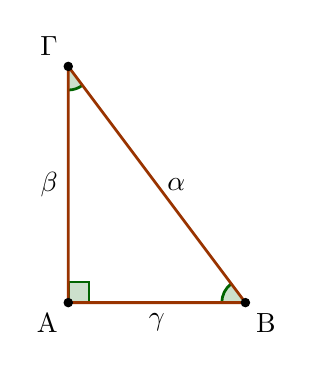
\begin{tikzpicture}[scale=.75]
\tkzSetUpLine[line width=1pt,color=black]
\tkzSetUpPoint[fill=black]

% Ορισμός των συντεταγμένων των κορυφών του τριγώνου.
\tkzDefPoints{0/0/A,3/0/B,0/4/C}

% Χρωματισμός του τριγώνου.
\tkzFillPolygon[fill=white](A,B,C)

% Επισήμανση γωνιών.
\tkzMarkRightAngle[line width=1pt, size=.35,color=AngleClr,fill=AngleClr,fill opacity=0.2](B,A,C)
\tkzFillAngles[fill=AngleClr,size=.4,fill opacity=0.2](C,B,A A,C,B)
\tkzMarkAngles[line width=1pt,size=.4,color=AngleClr](C,B,A A,C,B)

% Περίγραμμα του τριγώνου (προσοχή έρχεται μετά την επισήμανση των γωνιών).
\tkzDrawPolygon[color=ShapeClr](A,B,C)

% Επισήμανση σημείων.
\tkzDrawPoints[size=3](A,B,C)

% Ονόματα για τις κορυφές του τριγώνου.
\tkzLabelPoint[below left](A){$\mathrm{A}$}
\tkzLabelPoint[below right](B){$\mathrm{B}$}
\tkzLabelPoint[above left](C){$\mathrm{\Gamma}$}

% Ονόματα για τις πλευρές του τριγώνου.
\tkzLabelSegment[below](A,B){$\gamma$}
\tkzLabelSegment[left](A,C){$\beta$}
\tkzLabelSegment[right](B,C){$\alpha$}

\end{tikzpicture}
\end{document}